\section{Question 1}
We know inertia matrix is symetric so we have:
$$I_{xy} = I_{yx} = 10, \quad I_{xz} = I_{zx} = 0, \quad I_{yz} = I_{zy}$$

$$\boldsymbol{\mathrm{I}} = \begin{bmatrix}
    30 & -10 & 0 \\
    -10 & 20 & -I_{yz}\\
    0 & -I_{yz} & 30
\end{bmatrix}$$
\subsection{part a}
We know that:
\begin{equation}
    \boldsymbol{\mathrm{I}} \times \boldsymbol{\mathrm{\omega}} = \boldsymbol{\mathrm{h}}
\end{equation}

$$
\boldsymbol{\mathrm{\omega}} = \begin{bmatrix}
    10 & 10 & 10
\end{bmatrix}^T_{RPS} = \begin{bmatrix}
    10\times2\pi & 10\times2\pi & 10\times2\pi
\end{bmatrix}^T_{rad/\sec}, \quad \boldsymbol{\mathrm{h}} = \begin{bmatrix}
    200 & 200 & 400
\end{bmatrix}^T_{kg.m^2/s}
$$
If we use radian per second instead of revelotion per second $\boldsymbol{\mathrm{I}} \times \boldsymbol {\mathrm{\omega}} \neq \boldsymbol{\mathrm{h}}$ would happen.
$$ 
\boldsymbol{\mathrm{I}} \times \boldsymbol{\mathrm{\omega}} = \begin{bmatrix}
    200
    \\
    100 - 10I_{yz} \\
    300 - 10I_{yz}
\end{bmatrix} = \begin{bmatrix}
    200\\
    200\\
    400
\end{bmatrix} \rightarrow I_{yz} = -10 \rightarrow 
\boldsymbol{\mathrm{I}} = \begin{bmatrix}
    30 & -10 & 0 \\
    -10 & 20 & 10\\
    0 & 10 & 30
\end{bmatrix}
$$

\begin{equation}
T_{Rotational} = \dfrac{1}{2}\boldsymbol{\mathrm{\omega}}^T\times \boldsymbol{\mathrm{I}} \times \boldsymbol{\mathrm{\omega}} = \dfrac{1}{2} \begin{bmatrix}
    10&
    10&
    10
\end{bmatrix}\times
\begin{bmatrix}
    30 & -10 & 0 \\
    -10 & 20 & 10\\
    0 & 10 & 30
\end{bmatrix}\times
\begin{bmatrix}
    10\\
    10\\
    10
\end{bmatrix} = 4000
\end{equation}
\subsection{part b}
\begin{equation}
    T_{Rotational} = \dfrac{1}{2} \mathrm{I}_{\xi} \omega^2 \rightarrow \mathrm{I}_{\xi} = \dfrac{2T_{Rotational}}{\omega^2} = \dfrac{2\times 4000}{300} = 26.67
\end{equation}

Rotation matrix calculated via eigen vector of inertia matrix (used MATLAB to calculate).
\begin{equation}
    \boldsymbol{\mathrm{A}} = \mathrm{eig}(\boldsymbol{\mathrm{I}}) = \begin{bmatrix}
        -0.4082&   -0.7071&   -0.5774\\
        -0.8165&   -0.0000&    0.5774\\
         0.4082&   -0.7071&    0.5774\\
    \end{bmatrix}
\end{equation}

$$
\boldsymbol{\mathrm{I}}' = \boldsymbol{\mathrm{A}}^T \times \boldsymbol{\mathrm{I}} \times \boldsymbol{\mathrm{A}} = \begin{bmatrix}
    10 & 0  & 0 \\
    0  & 30 & 0\\
    0  & 0  & 40
\end{bmatrix}, \quad \boldsymbol{\mathrm{\omega}}' = \boldsymbol{\mathrm{A}}^T \boldsymbol{\mathrm{\omega}} = \begin{bmatrix}
    -8.1650\\
    -14.1421\\
      5.7735
\end{bmatrix}
$$

$$
h = |\boldsymbol{\mathrm{I}} \times \boldsymbol{\mathrm{\omega}}| = 489.8979
$$

We know that above matrix shows the direction cosines of the principal axes with the primary body axes. Used MATLAB function (dcm2angle) to calculate euler angles between two corinate system.
$$
\begin{bmatrix}
    \phi\\
    \theta\\
    \psi 
\end{bmatrix} = \begin{bmatrix}
  \ang{45.00}\\
  \ang{35.26}\\
  \ang{-120.00}
\end{bmatrix}
$$

\subsection{part c}
Ellipsoid of inertia calculated as folow:
\begin{equation}
    \dfrac{X^2}{\left(\sqrt{\dfrac{1}{\mathrm{I}_x}}\right)^2} + 
    \dfrac{Y^2}{\left(\sqrt{\dfrac{1}{\mathrm{I}_y}}\right)^2} + 
    \dfrac{Z^2}{\left(\sqrt{\dfrac{1}{\mathrm{I}_z}}\right)^2} =
    \dfrac{X^2}{\left(\sqrt{\dfrac{1}{10}}\right)^2} + 
    \dfrac{Y^2}{\left(\sqrt{\dfrac{1}{30}}\right)^2} + 
    \dfrac{Z^2}{\left(\sqrt{\dfrac{1}{40}}\right)^2} =
     1
\end{equation} 

\begin{figure}[H]
    \caption{ellipsoid of inertia}
    \centering
    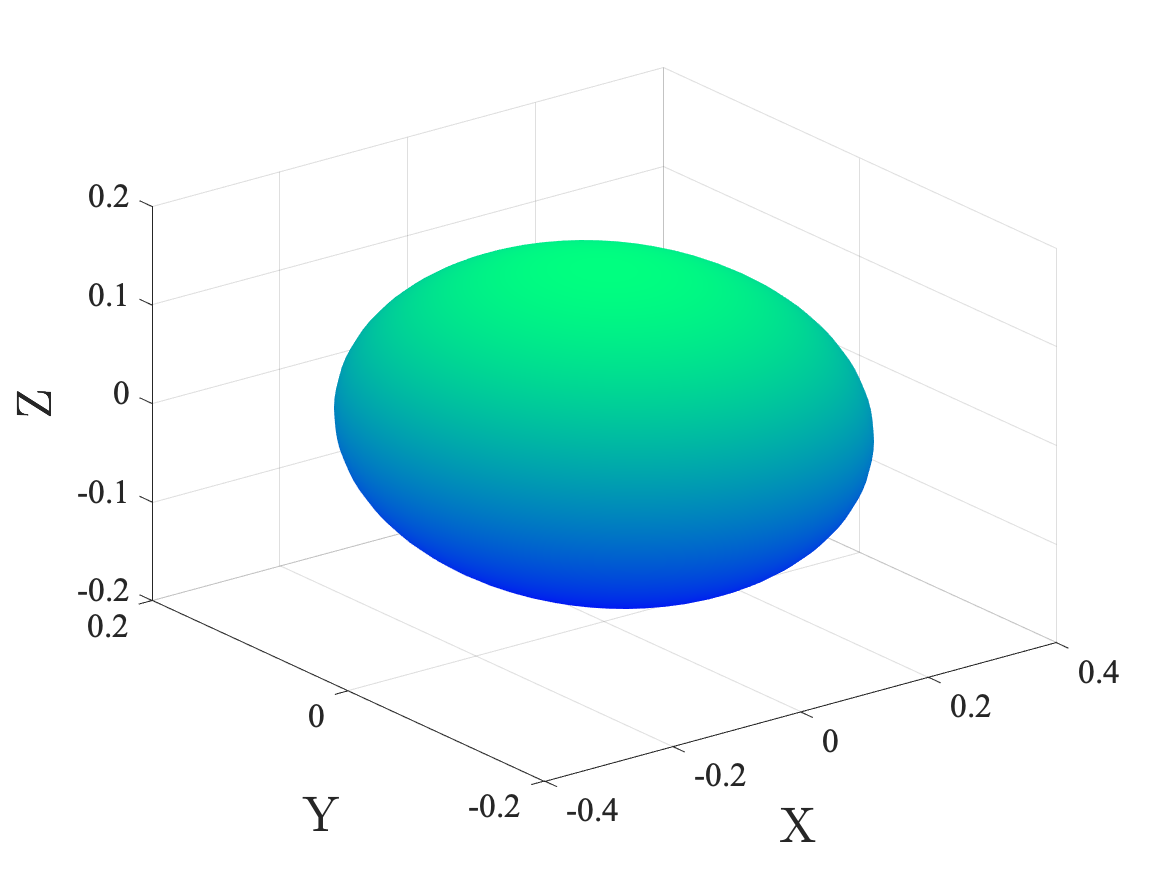
\includegraphics[width=17cm]{../Figure/Q1/3Dof_view_elipsoid_inertia}
\end{figure}

\begin{figure}[H]
    \caption{ellipsoid of inertia in zx plane}
    \centering
    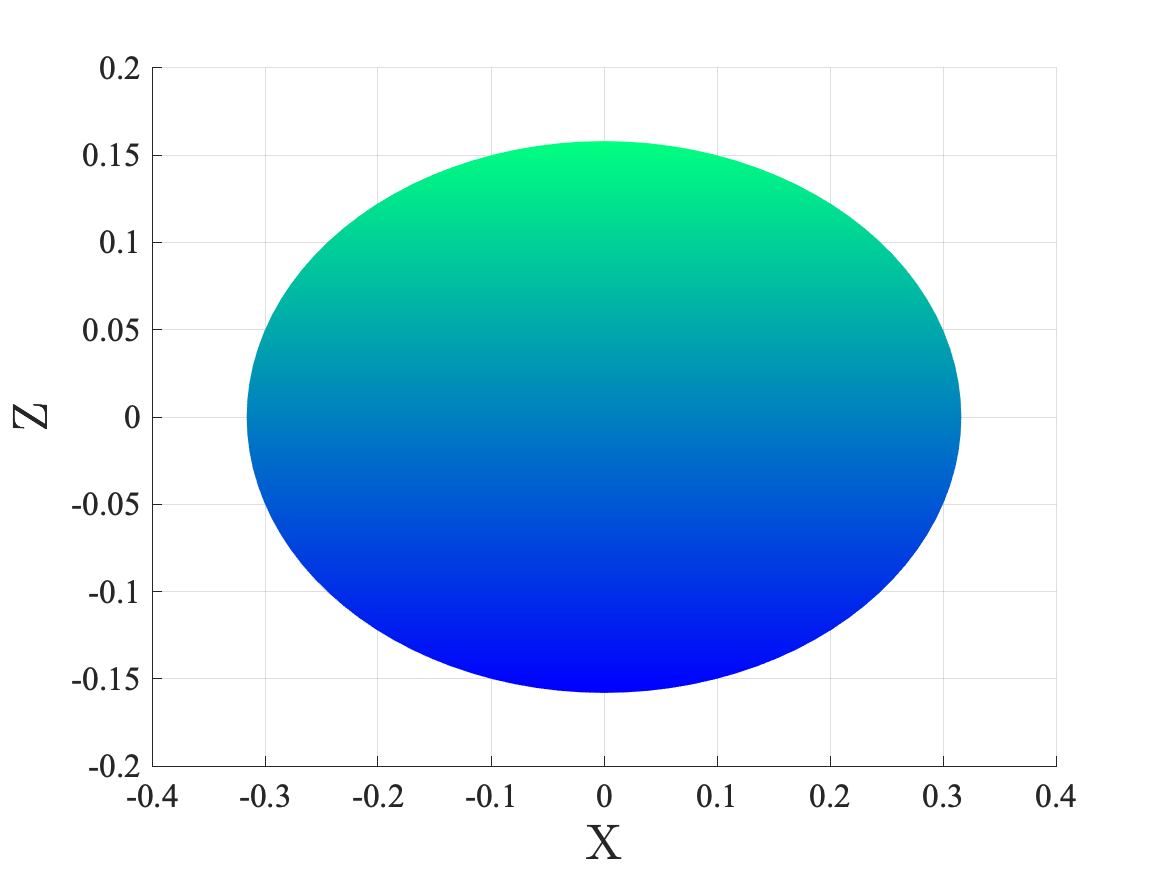
\includegraphics[width=12cm]{../Figure/Q1/xz_view_elipsoid_inertia}
\end{figure}

\begin{figure}[H]
    \caption{ellipsoid of inertia zy plane}
    \centering
    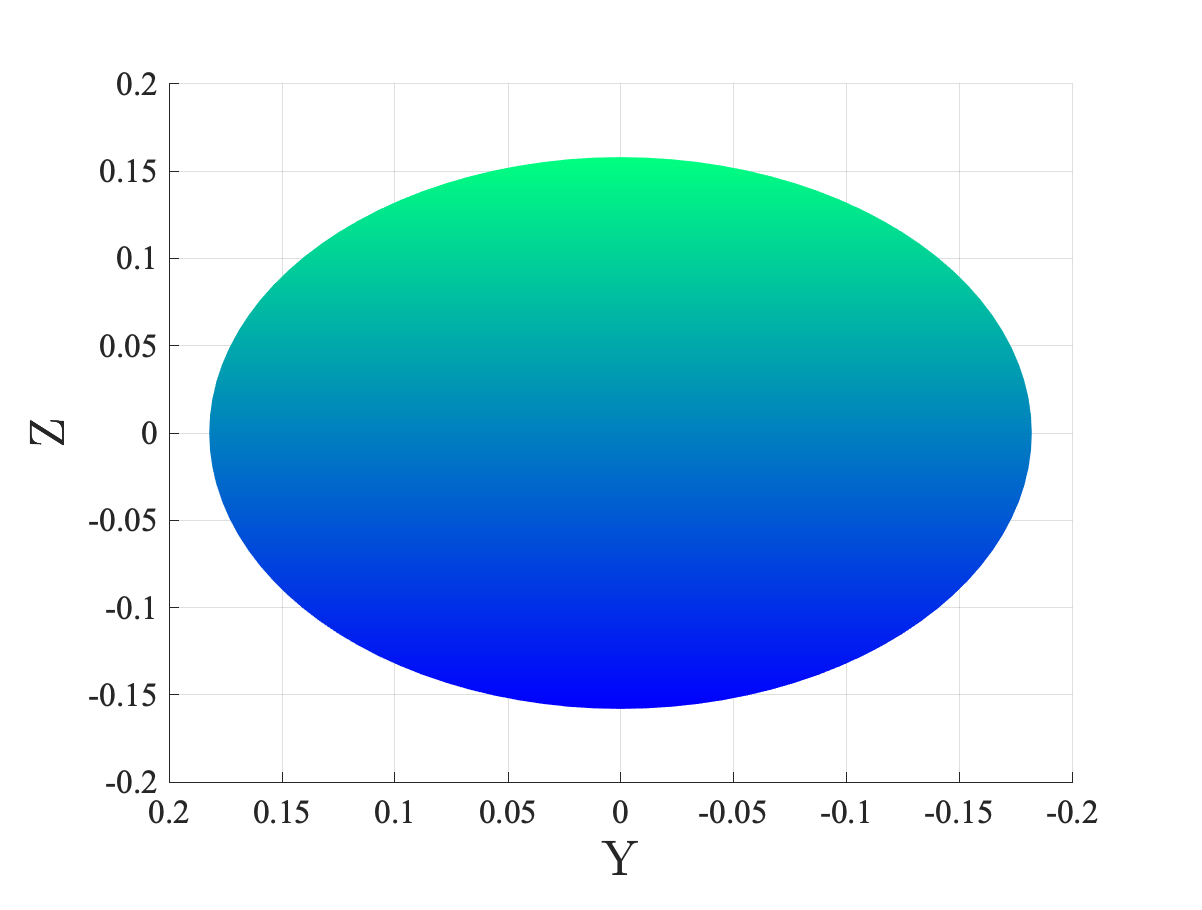
\includegraphics[width=12cm]{../Figure/Q1/yz_view_elipsoid_inertia}
\end{figure}

\begin{figure}[H]
    \caption{ellipsoid of inertia in xy plane}
    \centering
    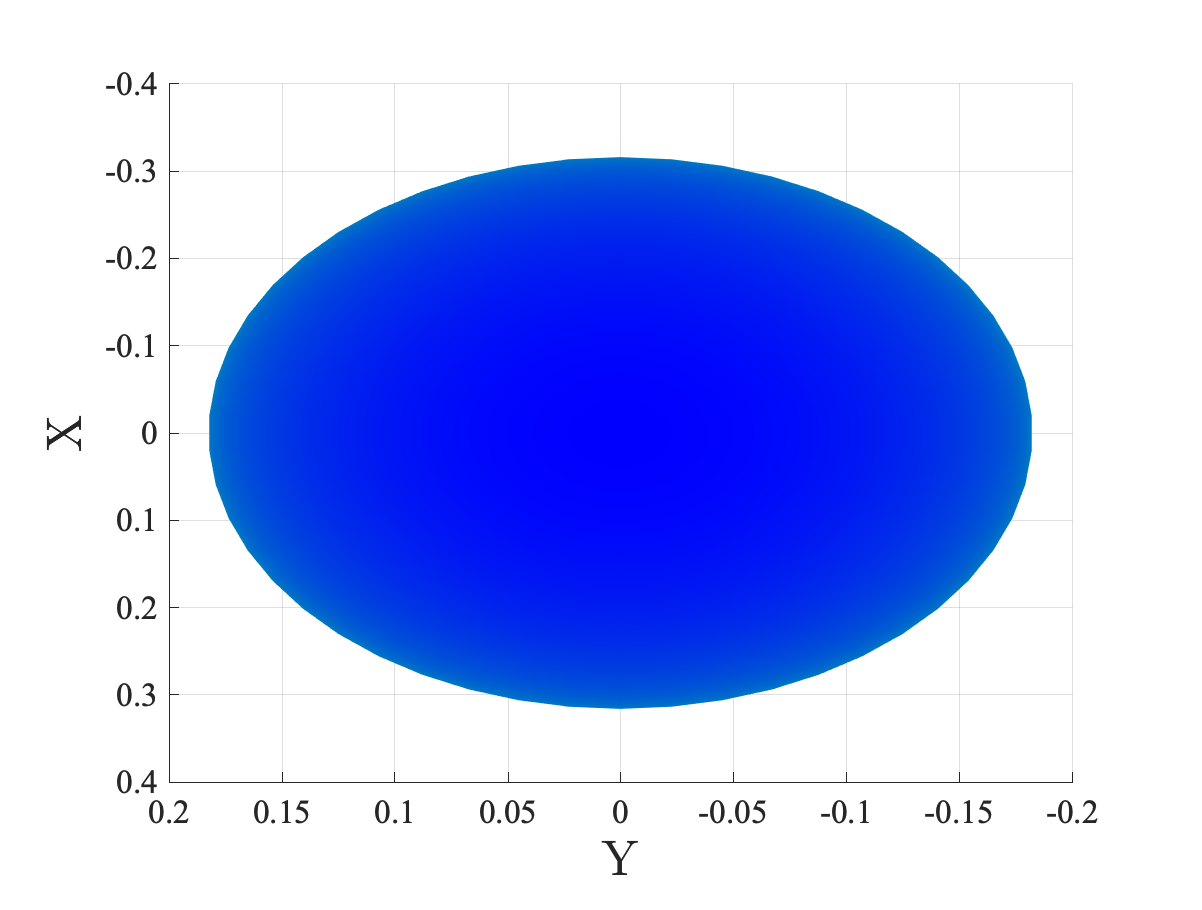
\includegraphics[width=12cm]{../Figure/Q1/xy_view_elipsoid_inertia}
\end{figure}

\subsection{part d}

Angular momentum and rotational kinetic energy ellipsoid calculated as folow:

\begin{equation}
    \dfrac{\omega_x^2}{\left(\dfrac{h}{\mathrm{I}_x}\right)^2} +
    \dfrac{\omega_y^2}{\left(\dfrac{h}{\mathrm{I}_y}\right)^2} +
    \dfrac{\omega_z^2}{\left(\dfrac{h}{\mathrm{I}_z}\right)^2} =
    \dfrac{\omega_x^2}{\left(\dfrac{490}{10}\right)^2} +
    \dfrac{\omega_y^2}{\left(\dfrac{490}{30}\right)^2} +
    \dfrac{\omega_z^2}{\left(\dfrac{490}{40}\right)^2} =
     1
\end{equation}


\begin{equation}
    \dfrac{\omega_x^2}{\left(\sqrt{\dfrac{2T}{\mathrm{I}_x}}\right)^2} +
    \dfrac{\omega_y^2}{\left(\sqrt{\dfrac{2T}{\mathrm{I}_y}}\right)^2} +
    \dfrac{\omega_z^2}{\left(\sqrt{\dfrac{2T}{\mathrm{I}_z}}\right)^2} =
    \dfrac{\omega_x^2}{\left(\sqrt{\dfrac{2\times 4000}{10}}\right)^2} +
    \dfrac{\omega_y^2}{\left(\sqrt{\dfrac{2\times 4000}{30}}\right)^2} +
    \dfrac{\omega_z^2}{\left(\sqrt{\dfrac{2\times 4000}{40}}\right)^2} = 1
\end{equation}

Ellipsoid parameter calculated before, now, use them to draw the ellipsoid.

\begin{figure}[H]
    \caption{Angular momentum and rotational kinetic energy ellipsoid of inertia}
    \centering
    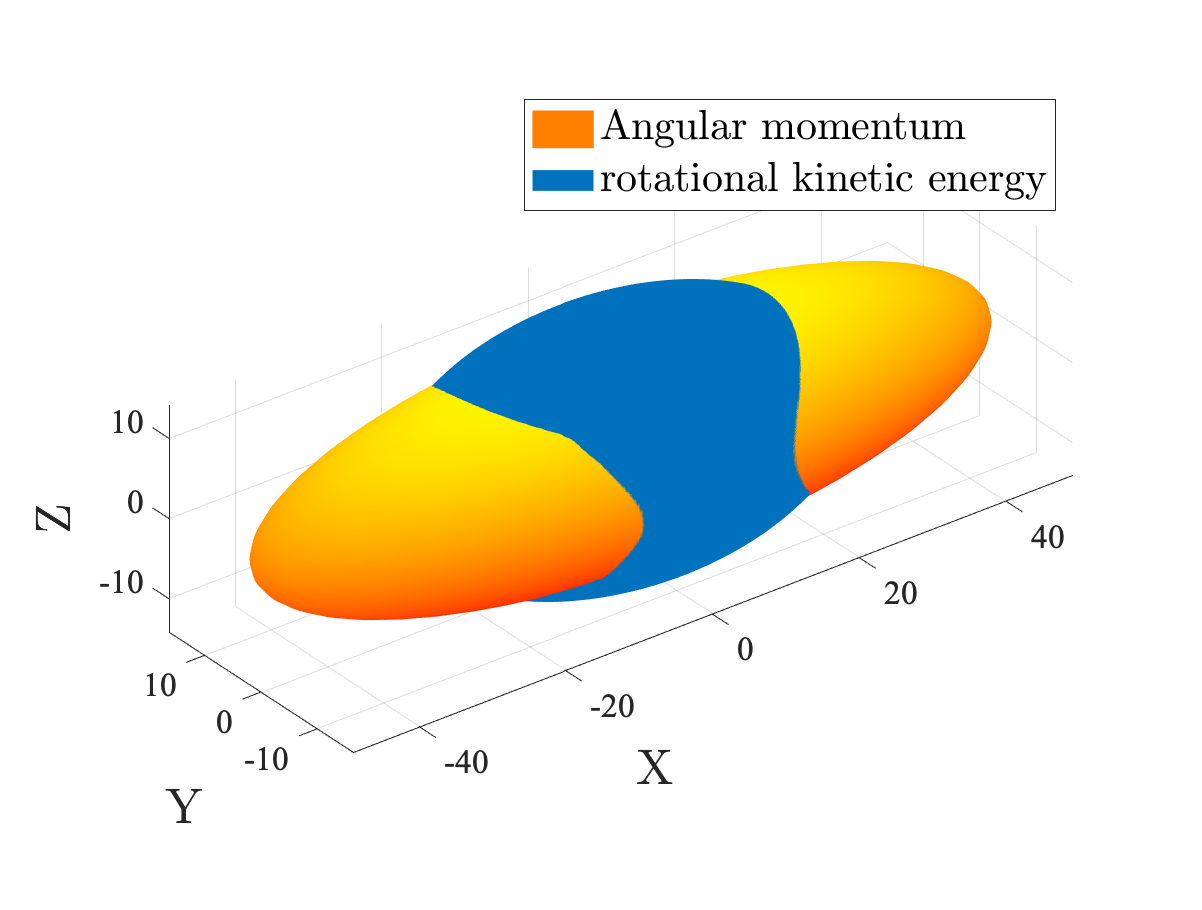
\includegraphics[width=16cm]{../Figure/Q1/3Dof_view}
\end{figure}
\vspace{-1.5cm}
\begin{figure}[H]
    \caption{Angular momentum and rotational kinetic energy ellipsoid of inertia in zx plane}
    \centering
    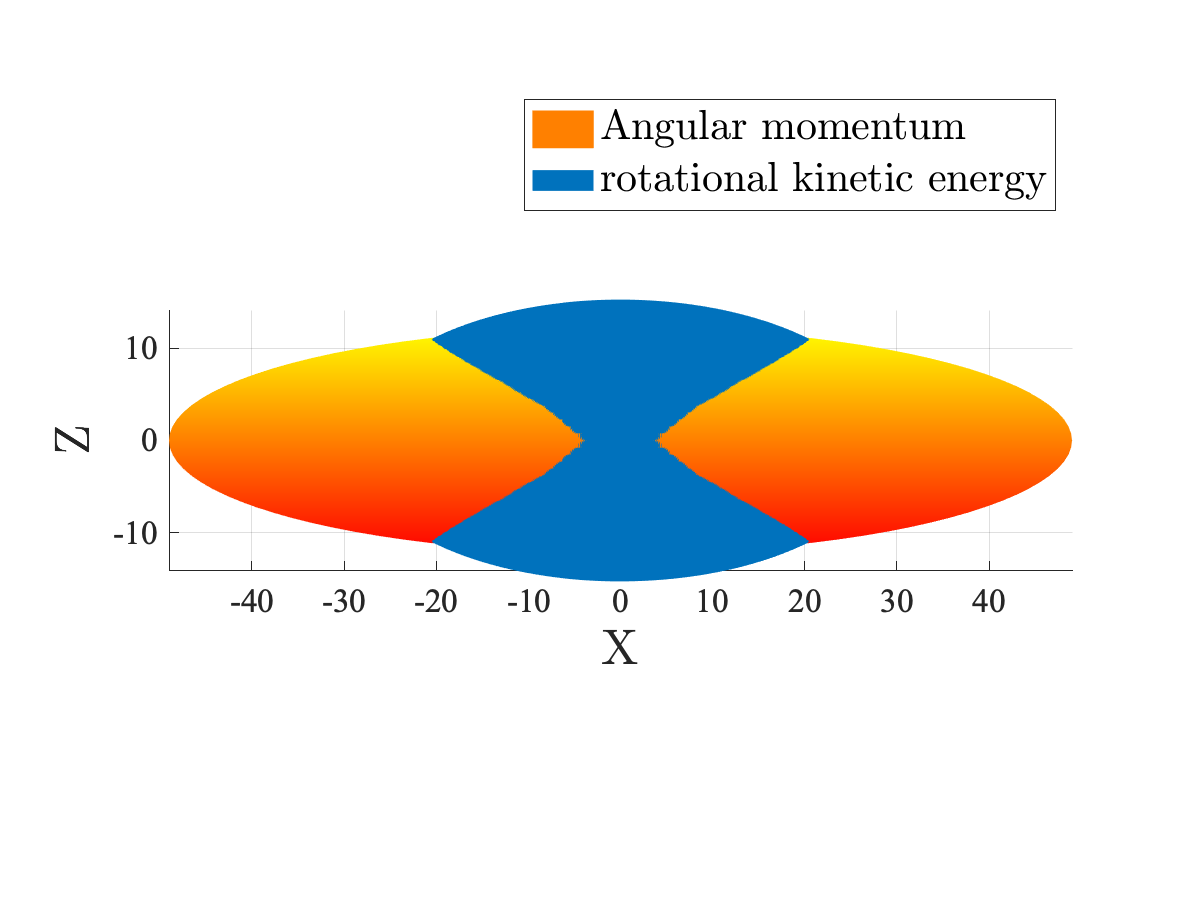
\includegraphics[width=12cm]{../Figure/Q1/xz_view}
\end{figure}

\begin{figure}[H]
    \caption{Angular momentum and rotational kinetic energy ellipsoid of inertia zy plane}
    \centering
    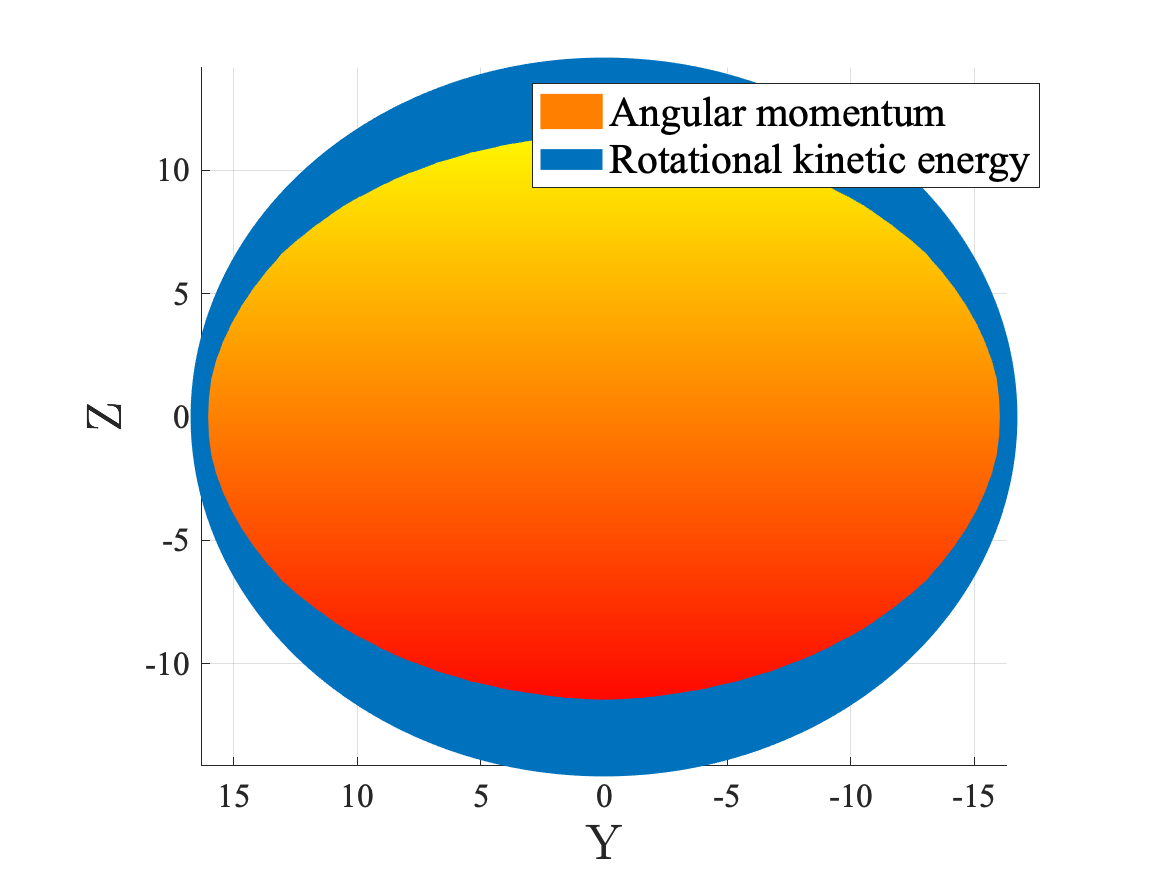
\includegraphics[width=12cm]{../Figure/Q1/yz_view}
\end{figure}

\begin{figure}[H]
    \caption{Angular momentum and rotational kinetic energy ellipsoid of inertia in xy plane}
    \centering
    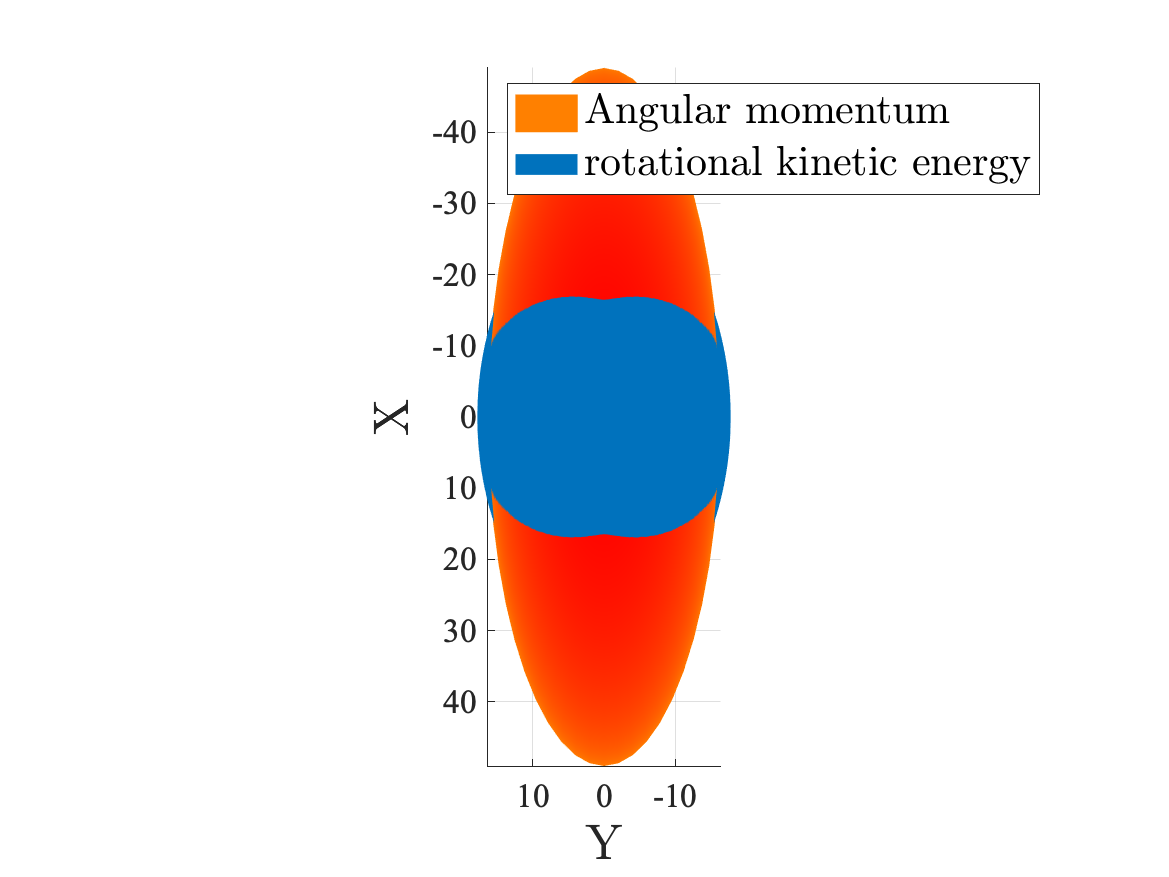
\includegraphics[width=12cm]{../Figure/Q1/xy_view}
\end{figure}

\subsection{Bonus}

\begin{equation}
    \dfrac{\omega_x^2}{\left(\dfrac{h}{\mathrm{I}_x}\right)^2} +
    \dfrac{\omega_y^2}{\left(\dfrac{h}{\mathrm{I}_y}\right)^2} +
    \dfrac{\omega_z^2}{\left(\dfrac{h}{\mathrm{I}_z}\right)^2} = 1 \to \omega_x^2 = -\dfrac{\left(\dfrac{h}{\mathrm{I}_x}\right)^2\omega_y^2}{\left(\dfrac{h}{\mathrm{I}_y}\right)^2} -
    \dfrac{\left(\dfrac{h}{\mathrm{I}_x}\right)^2\omega_z^2}{\left(\dfrac{h}{\mathrm{I}_z}\right)^2} + \left(\dfrac{h}{\mathrm{I}_x}\right)^2
\end{equation}


\begin{equation}
    \dfrac{\omega_x^2}{\left(\sqrt{\dfrac{2T}{\mathrm{I}_x}}\right)^2} +
    \dfrac{\omega_y^2}{\left(\sqrt{\dfrac{2T}{\mathrm{I}_y}}\right)^2} +
    \dfrac{\omega_z^2}{\left(\sqrt{\dfrac{2T}{\mathrm{I}_z}}\right)^2} = 1 \to     \dfrac{-\dfrac{\left(\dfrac{h}{\mathrm{I}_x}\right)^2\omega_y^2}{\left(\dfrac{h}{\mathrm{I}_y}\right)^2} -
    \dfrac{\left(\dfrac{h}{\mathrm{I}_x}\right)^2\omega_z^2}{\left(\dfrac{h}{\mathrm{I}_z}\right)^2} + \left(\dfrac{h}{\mathrm{I}_x}\right)^2}{\left(\sqrt{\dfrac{2T}{\mathrm{I}_x}}\right)^2} +
    \dfrac{\omega_y^2}{\left(\sqrt{\dfrac{2T}{\mathrm{I}_y}}\right)^2} +
    \dfrac{\omega_z^2}{\left(\sqrt{\dfrac{2T}{\mathrm{I}_z}}\right)^2} = 1
\end{equation}

\begin{equation}
    \to -\dfrac{\left(\dfrac{h}{\mathrm{I}_x}\right)^2\omega_y^2}{\left(\dfrac{h}{\mathrm{I}_y}\right)^2} -
    \dfrac{\left(\dfrac{h}{\mathrm{I}_x}\right)^2\omega_z^2}{\left(\dfrac{h}{\mathrm{I}_z}\right)^2} + \left(\dfrac{h}{\mathrm{I}_x}\right)^2 +
    \dfrac{\left(\sqrt{\dfrac{2T}{\mathrm{I}_x}}\right)^2\omega_y^2}{\left(\sqrt{\dfrac{2T}{\mathrm{I}_y}}\right)^2} +
    \dfrac{\left(\sqrt{\dfrac{2T}{\mathrm{I}_x}}\right)^2\omega_z^2}{\left(\sqrt{\dfrac{2T}{\mathrm{I}_z}}\right)^2} =\left(\sqrt{\dfrac{2T}{\mathrm{I}_x}}\right)^2
\end{equation}

\begin{equation}
    \omega^2_y \left(-\dfrac{\left(\dfrac{h}{\mathrm{I}_x}\right)^2}{\left(\dfrac{h}{\mathrm{I}_y}\right)^2}+\dfrac{\left(\sqrt{\dfrac{2T}{\mathrm{I}_x}}\right)^2}{\left(\sqrt{\dfrac{2T}{\mathrm{I}_y}}\right)^2} \right) + \omega_z^2\left(-\dfrac{\left(\dfrac{h}{\mathrm{I}_x}\right)^2}{\left(\dfrac{h}{\mathrm{I}_z}\right)^2}+\dfrac{\left(\sqrt{\dfrac{2T}{\mathrm{I}_x}}\right)^2}{\left(\sqrt{\dfrac{2T}{\mathrm{I}_z}}\right)^2} \right) = \left(\sqrt{\dfrac{2T}{\mathrm{I}_x}}\right)^2 - \left(\dfrac{h}{\mathrm{I}_x}\right)^2
\end{equation}

\begin{equation}
    \omega_y^2\left(\dfrac{\mathrm{I}_y}{\mathrm{I}_x} - \dfrac{\mathrm{I}_y^2}{\mathrm{I}_x^2} \right) +
    \omega_z^2\left(\dfrac{\mathrm{I}_z}{\mathrm{I}_x} - \dfrac{\mathrm{I}_z^2}{\mathrm{I}_x^2} \right) = \left(\sqrt{\dfrac{2T}{\mathrm{I}_x}}\right)^2 - \left(\dfrac{h}{\mathrm{I}_x}\right)^2
\end{equation}

Mathematical formulas for the Polhode curves is a ellipsoid in yz plane.